\documentclass[journal,12pt,twocolumn]{IEEEtran}
\usepackage{setspace}
\usepackage{gensymb}
\usepackage{caption}
%\usepackage{multirow}
%\usepackage{multicolumn}
%\usepackage{subcaption}
%\doublespacing
\singlespacing
\usepackage{csvsimple}
\usepackage{amsmath}
\usepackage{multicol}
%\usepackage{enumerate}
\usepackage{amssymb}
%\usepackage{graphicx}
\usepackage{newfloat}
%\usepackage{syntax}
\usepackage{listings}
%\usepackage{iithtlc}
\usepackage{color}
\usepackage{tikz}
\usetikzlibrary{shapes,arrows}



%\usepackage{graphicx}
%\usepackage{amssymb}
%\usepackage{relsize}
%\usepackage[cmex10]{amsmath}
%\usepackage{mathtools}
%\usepackage{amsthm}
%\interdisplaylinepenalty=2500
%\savesymbol{iint}
%\usepackage{txfonts}
%\restoresymbol{TXF}{iint}
%\usepackage{wasysym}
\usepackage{amsthm}
\usepackage{mathrsfs}
\usepackage{txfonts}
\usepackage{stfloats}
\usepackage{cite}
\usepackage{cases}
\usepackage{mathtools}
\usepackage{caption}
\usepackage{enumerate}	
\usepackage{enumitem}
\usepackage{amsmath}
%\usepackage{xtab}
\usepackage{longtable}
\usepackage{multirow}
%\usepackage{algorithm}
%\usepackage{algpseudocode}
\usepackage{enumitem}
\usepackage{mathtools}
\usepackage{hyperref}
%\usepackage[framemethod=tikz]{mdframed}
\usepackage{listings}

\usepackage{tikz}
\usetikzlibrary{shapes.geometric,calc,angles,positioning,intersections,quotes,decorations,babel,patterns,fit}
\usepackage{tkz-euclide}
\usetkzobj{all}
    %\usepackage[latin1]{inputenc}                                 %%
    \usepackage{color}                                            %%
    \usepackage{array}                                            %%
    \usepackage{longtable}                                        %%
    \usepackage{calc}                                             %%
    \usepackage{multirow}                                         %%
    \usepackage{hhline}                                           %%
    \usepackage{ifthen}                                           %%
  %optionally (for landscape tables embedded in another document): %%
    \usepackage{lscape}     


\usepackage{url}
\def\UrlBreaks{\do\/\do-}


%\usepackage{stmaryrd}


%\usepackage{wasysym}
%\newcounter{MYtempeqncnt}
\DeclareMathOperator*{\Res}{Res}
%\renewcommand{\baselinestretch}{2}
\renewcommand\thesection{\arabic{section}}
\renewcommand\thesubsection{\thesection.\arabic{subsection}}
\renewcommand\thesubsubsection{\thesubsection.\arabic{subsubsection}}

\renewcommand\thesectiondis{\arabic{section}}
\renewcommand\thesubsectiondis{\thesectiondis.\arabic{subsection}}
\renewcommand\thesubsubsectiondis{\thesubsectiondis.\arabic{subsubsection}}

% correct bad hyphenation here
\hyphenation{op-tical net-works semi-conduc-tor}

%\lstset{
%language=C,
%frame=single, 
%breaklines=true
%}

%\lstset{
	%%basicstyle=\small\ttfamily\bfseries,
	%%numberstyle=\small\ttfamily,
	%language=Octave,
	%backgroundcolor=\color{white},
	%%frame=single,
	%%keywordstyle=\bfseries,
	%%breaklines=true,
	%%showstringspaces=false,
	%%xleftmargin=-10mm,
	%%aboveskip=-1mm,
	%%belowskip=0mm
%}

%\surroundwithmdframed[width=\columnwidth]{lstlisting}
\def\inputGnumericTable{}                                 %%
\lstset{
%language=C,
frame=single, 
breaklines=true,
columns=fullflexible
}
 

\begin{document}
%
\tikzstyle{block} = [rectangle, draw,
    text width=3em, text centered, minimum height=3em]
\tikzstyle{sum} = [draw, circle, node distance=3cm]
\tikzstyle{input} = [coordinate]
\tikzstyle{output} = [coordinate]
\tikzstyle{pinstyle} = [pin edge={to-,thin,black}]

\theoremstyle{definition}
\newtheorem{theorem}{Theorem}[section]
\newtheorem{problem}{Problem}
\newtheorem{proposition}{Proposition}[section]
\newtheorem{lemma}{Lemma}[section]
\newtheorem{corollary}[theorem]{Corollary}
\newtheorem{example}{Example}[section]
\newtheorem{definition}{Definition}[section]
%\newtheorem{algorithm}{Algorithm}[section]
%\newtheorem{cor}{Corollary}
\newcommand{\BEQA}{\begin{eqnarray}}
\newcommand{\EEQA}{\end{eqnarray}}
\newcommand{\define}{\stackrel{\triangle}{=}}

\bibliographystyle{IEEEtran}
%\bibliographystyle{ieeetr}

\providecommand{\nCr}[2]{\,^{#1}C_{#2}} % nCr
\providecommand{\nPr}[2]{\,^{#1}P_{#2}} % nPr
\providecommand{\mbf}{\mathbf}
\providecommand{\pr}[1]{\ensuremath{\Pr\left(#1\right)}}
\providecommand{\qfunc}[1]{\ensuremath{Q\left(#1\right)}}
\providecommand{\sbrak}[1]{\ensuremath{{}\left[#1\right]}}
\providecommand{\lsbrak}[1]{\ensuremath{{}\left[#1\right.}}
\providecommand{\rsbrak}[1]{\ensuremath{{}\left.#1\right]}}
\providecommand{\brak}[1]{\ensuremath{\left(#1\right)}}
\providecommand{\lbrak}[1]{\ensuremath{\left(#1\right.}}
\providecommand{\rbrak}[1]{\ensuremath{\left.#1\right)}}
\providecommand{\cbrak}[1]{\ensuremath{\left\{#1\right\}}}
\providecommand{\lcbrak}[1]{\ensuremath{\left\{#1\right.}}
\providecommand{\rcbrak}[1]{\ensuremath{\left.#1\right\}}}
\theoremstyle{remark}
\newtheorem{rem}{Remark}
\newcommand{\sgn}{\mathop{\mathrm{sgn}}}
\providecommand{\abs}[1]{\left\vert#1\right\vert}
\providecommand{\res}[1]{\Res\displaylimits_{#1}} 
\providecommand{\norm}[1]{\left\Vert#1\right\Vert}
\providecommand{\mtx}[1]{\mathbf{#1}}
\providecommand{\mean}[1]{E\left[ #1 \right]}
\providecommand{\fourier}{\overset{\mathcal{F}}{ \rightleftharpoons}}
%\providecommand{\hilbert}{\overset{\mathcal{H}}{ \rightleftharpoons}}
\providecommand{\system}{\overset{\mathcal{H}}{ \longleftrightarrow}}
	%\newcommand{\solution}[2]{\textbf{Solution:}{#1}}
\newcommand{\solution}{\noindent \textbf{Solution: }}
\newcommand{\myvec}[1]{\ensuremath{\begin{pmatrix}#1\end{pmatrix}}}
\providecommand{\dec}[2]{\ensuremath{\overset{#1}{\underset{#2}{\gtrless}}}}
\DeclarePairedDelimiter{\ceil}{\lceil}{\rceil}
%\numberwithin{equation}{section}
%\numberwithin{problem}{subsection}
%\numberwithin{definition}{subsection}
\makeatletter
\@addtoreset{figure}{section}
\makeatother

\let\StandardTheFigure\thefigure
%\renewcommand{\thefigure}{\theproblem.\arabic{figure}}
\renewcommand{\thefigure}{\thesection}


%\numberwithin{figure}{subsection}

%\numberwithin{equation}{subsection}
%\numberwithin{equation}{section}
%\numberwithin{equation}{problem}
%\numberwithin{problem}{subsection}
\numberwithin{problem}{section}
%%\numberwithin{definition}{subsection}
%\makeatletter
%\@addtoreset{figure}{problem}
%\makeatother
\makeatletter
\@addtoreset{table}{section}
\makeatother

\let\StandardTheFigure\thefigure
\let\StandardTheTable\thetable
\let\vec\mathbf
%%\renewcommand{\thefigure}{\theproblem.\arabic{figure}}
%\renewcommand{\thefigure}{\theproblem}

%%\numberwithin{figure}{section}

%%\numberwithin{figure}{subsection}



\def\putbox#1#2#3{\makebox[0in][l]{\makebox[#1][l]{}\raisebox{\baselineskip}[0in][0in]{\raisebox{#2}[0in][0in]{#3}}}}
     \def\rightbox#1{\makebox[0in][r]{#1}}
     \def\centbox#1{\makebox[0in]{#1}}
     \def\topbox#1{\raisebox{-\baselineskip}[0in][0in]{#1}}
     \def\midbox#1{\raisebox{-0.5\baselineskip}[0in][0in]{#1}}

\vspace{3cm}

\title{ 
%	\logo{
GEOMETRY
%	}
}


	
	

\maketitle

%\tableofcontents

\bigskip

\renewcommand{\thefigure}{\theenumi}
\renewcommand{\thetable}{\theenumi}


\begin{enumerate}[label=\arabic*]
\numberwithin{equation}{enumi}


\item Construct a tangent to a circle of radius 4 units
from a point on the concentric circle of radius
6 units.\\
\begin{itemize}
\item\textbf{Solution} :\\\\
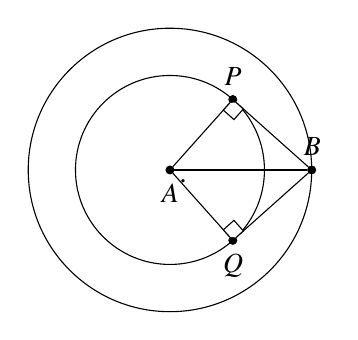
\begin{tikzpicture}
[scale =0.3,>=stealth,point/.style = {draw, circle, fill = black, inner sep = 1pt},]
\node (A) at (0,0)[point,label=below :$A$] {};
\node (P) at (2.66,2.98)[point,label=above :$P$] {};
\node (B) at (6,0)[point,label=above :$B$] {};
\node (Q) at (2.66,-2.98)[point,label=below :$Q$] {};
\draw (0,0) node [below right] {.} circle (6);
\draw (0,0) node [below right] {.} circle (4);
\draw (B)--(A);
\draw (B)--(Q);
\draw (B)--(P);
\draw (A)--(P);
\draw (A)--(Q);
\tkzMarkRightAngle[fill=white!45,size=.6,mark=](B,P,A)
\tkzMarkRightAngle[fill=white!45,size=.6,mark=](B,Q,A)
\end{tikzpicture}
\\
 PB and QB are the tangents 
\item \textbf{Given} : r1=4 and r2 = 6\\
\begin{align*}
a=\sqrt{r2^2 - r1^2}\\
a=4.47\\
c=r1 , b=r2\\
p=\frac{b^2+c^2-a^2}{2b}\\
p=2.66\\
q=\sqrt{c^2 - p^2}\\
q=2.98\\
AB = r2 \\
P = (2.66,2.98)\\
Q = (2.66,-2.98)
\end{align*}
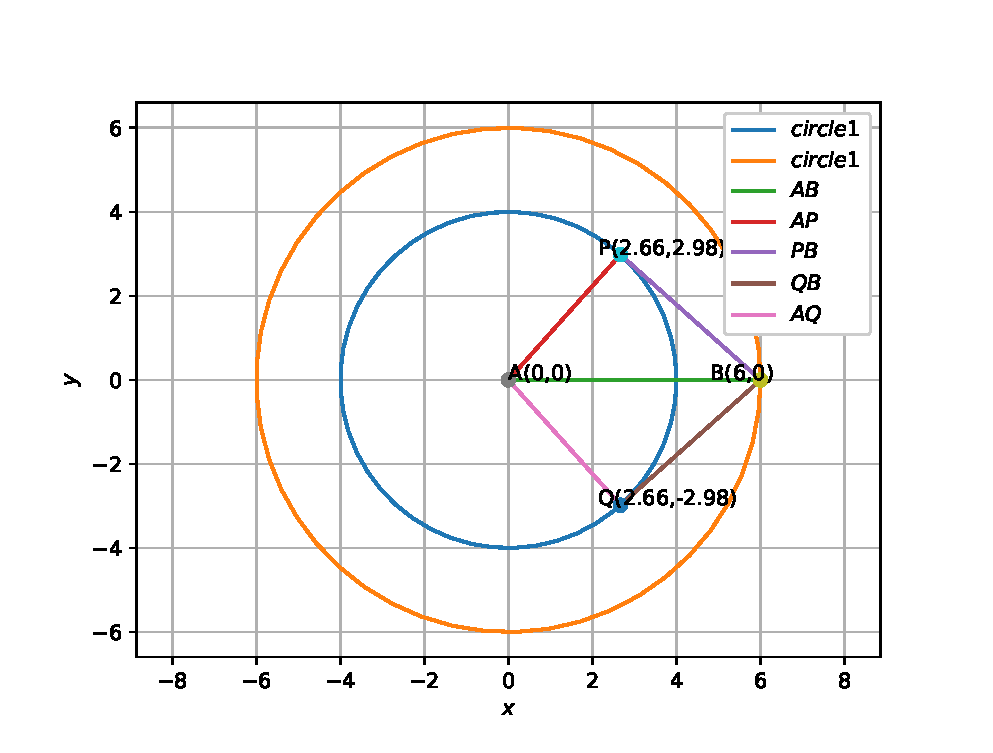
\includegraphics[scale=.4]{./figs/CIR_CON.eps}
\begin{lstlisting}
https://github.com/pratibha444/GEOMETRY/blob/master/figs/CIRCLE_CON.tex
\end{lstlisting}
\begin{lstlisting}
https://github.com/pratibha444/GEOMETRY/blob/master/CODES/circle/circon.py
\end{lstlisting}
\end{itemize}

\textbf{Triangle construction}\\

\item Construct an isosceles triangle in which the lengths of the equal sides is 6.5 and the angle between them is 110$\degree$
\begin{itemize}
\item\textbf{Solution}\\
\begin{tikzpicture}
[scale =0.6,>=stealth,point/.style = {draw, circle, fill = black, inner sep = 1pt},]
\node (B) at (0,0)[point,label=below :$B$] {};
\node (A) at (-2.223,6.108)[point,label=above :$A$] {};
\node (C) at (6.5,0)[point,label=below :$C$] {};
\draw (A)--(B);
\draw (B)--(C);
\draw (C)--(A);
\tkzMarkAngle[fill=green!40,size=0.5cm,mark=](C,B,A)
\tkzLabelAngle[pos=1](C,B,A){\rotatebox{-360}{$110$}}
\end{tikzpicture}

\item BC = 6.5 \item AC = 10.64
\item AB = 6.5
\item $\angle B$ = 110\\ 
\item\textbf{Given}: BC = 6.5 and AB = 6.5\\
$\angle$ABC = 110
\begin{align*}
a = 6.5 and  c = 6.5\\
b = \sqrt{a^2 + c^2 - 2ac cos(A)}\\
b= 10.64\\
p=\frac{a^2 + c^2 - b^2}{2a}\\
p=-2.22\\
q=\sqrt{c^2 - p^ 2}\\
q = 6.10
\end{align*}
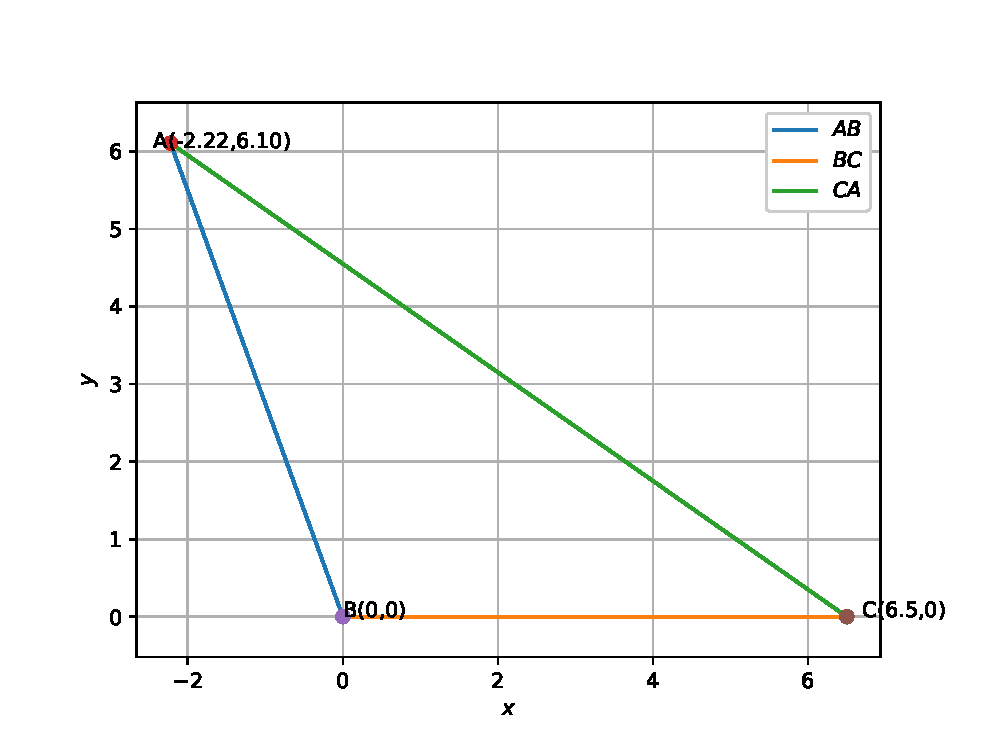
\includegraphics[scale=.4]{./figs/TRI_CON.eps}
\begin{lstlisting}
https://github.com/pratibha444/GEOMETRY/blob/master/figs/tri_iso.tex
\end{lstlisting}
\begin{lstlisting}
https://github.com/pratibha444/GEOMETRY/blob/master/CODES/triangle/TRI_CON.py
\end{lstlisting}
\end{itemize}





\textbf{Quadrilateral excercise}\\

\item A farmer was having a field in the form of a
parallelogram PQRS . She took any point A on
RS and joined it to points P and Q. In how
many parts the fields is divided? What are the
shapes of these parts? The farmer wants to sow
wheat and pulses in equal portions of the field
separately. How should she do it?
\begin{itemize}
\item \textbf{Solution} :
\begin{center}
\documentclass{article}
\usepackage{tikz}
\usetikzlibrary{shapes.geometric,calc,angles,positioning,intersections,quotes,decorations,babel,patterns,fit}
\usepackage{tkz-euclide}
\usetkzobj{all}
\begin{document}
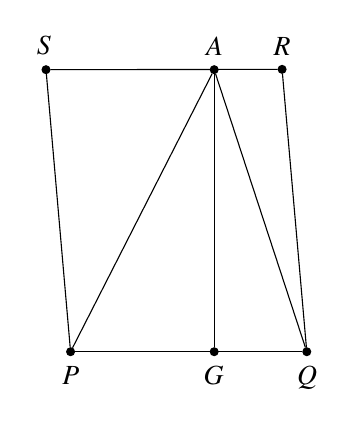
\begin{tikzpicture}
[scale =0.6,>=stealth,point/.style = {draw, circle, fill = black, inner sep = 1pt},]
\node (S) at (-0.52,5.97)[point,label=above :$S$] {};
\node (P) at (0,0)[point,label=below :$P$] {};
\node (A) at (3.04,5.97)[point,label=above :$A$] {};
\node (R) at (4.477,5.977)[point,label=above :$R$] {};
\node (G) at (3.04,0)[point,label=below:$G$] {};
\node (Q) at (5,0)[point,label=below :$Q$] {};
\draw (S)--(P);
\draw (P)--(Q);
\draw (Q)--(R);
\draw (R)--(S);
\draw (A)--(P);
\draw (A)--(Q);
\draw (A)--(G);
\end{tikzpicture}
\end{document}
\end{center}

\item S = (-0.52,5.97)\\
\item A = (3.04,5.97)\\
\item R = (4.47,5.57)
\item  Distance between S and A

\begin{align*}
z = \sqrt{(x_1 - x_2)^2 + (y_1 - y_2)^2}\\
z = \sqrt{(3.04 + 0.52) + (5.97 - 5.97)}\\
z = 3.55
\end{align*}

\item Distance between A and R

\begin{align*}
z = \sqrt{(x_1 - x_2)^2 + (y_1 - y_2)^2}\\
z = \sqrt{(4.47 - 3.04) + (5.97 - 5.97)}\\
z = 1.43
\end{align*}

\item PQ = 5\\
\item SP = 6\\
\item AG = 6\\
\item$\triangle$ APQ = $\triangle$PAS + $\triangle$ QAR\\ 
\item$\triangle$ APQ = $\frac{1}{2}$ X l X b\\
$\triangle$ APQ = $\frac{1}{2}$ X 6 X 5\\
$\triangle$ APQ = 15$cm^2$
\item$\triangle$ PAS = $\frac{1}{2}$ X l X b\\
$\triangle$ PAS = $\frac{1}{2}$ X 6 X 3.55\\
$\triangle$ PAS = 10.65$cm^2$\\
\item$\triangle$ QRA = $\frac{1}{2}$ X l X b\\
$\triangle$ QRA = $\frac{1}{2}$ X 6 X 1.43\\
$\triangle$ QRA = 4.38$cm^2$\\
\item 10.65 + 4.38 = 15
\item Hence Area of $\triangle$APQ = Area of $\triangle$PAS + Area of $\triangle$QAR\\

\item  After joining the point A to p and Q, the feild is divided into 3 parts.\\
\item All the three parts are in triangle shape.\\
As PQRS is a parallelogram so\\

Area of PQRS = (Area of $\triangle$APS + $\triangle$ARQ + $\triangle$PAQ) --(1)\\
Area of triangle is half of parallelogram\\
if they have same base and lie between same parallel lines. \\
Area of $\triangle$PAQ = $\frac{1}{2}$ Area of PQRS\\
$\triangle$PAQ = $\frac{1}{2}$area($\triangle$APS + $\triangle$ARQ + $\triangle$APQ\\
2$\triangle$PAQ - $\triangle$PAQ = area($\triangle$APS + $\triangle$ARQ)\\
$\triangle$PAQ = $\triangle$APS + $\triangle$ARQ\\

Hence the farmer can sow wheat in $\triangle$PAQ and pulses in $\triangle$APS and $\triangle$ARQ\\

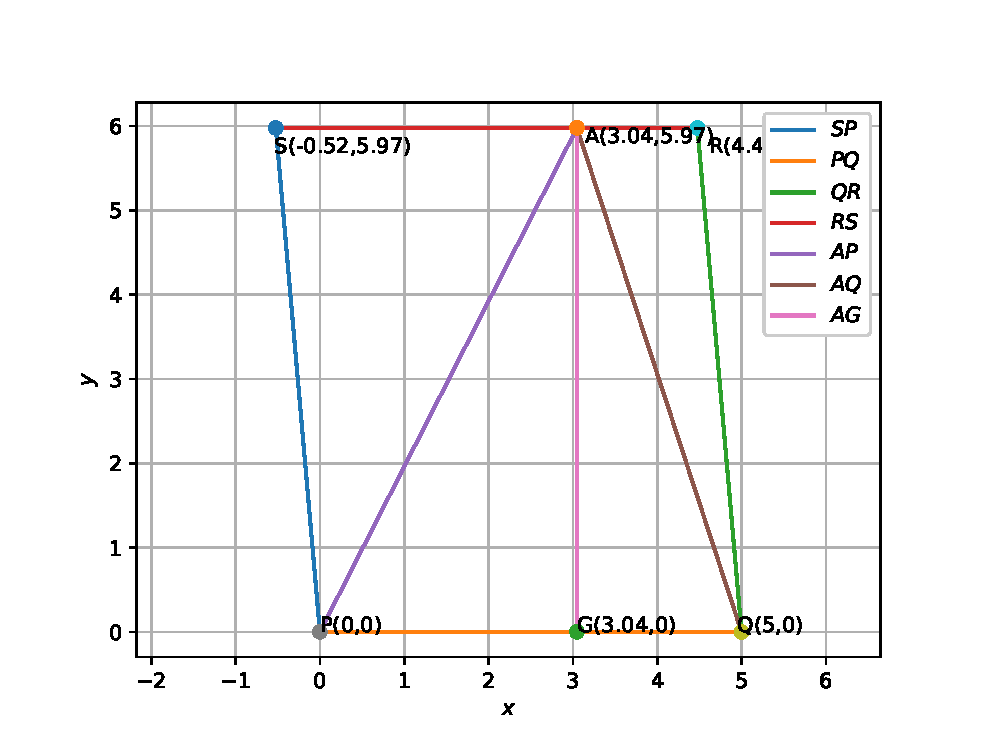
\includegraphics[scale=.5]{./figs/farme.eps}\\
\begin{lstlisting}
https://github.com/pratibha444/GEOMETRY/blob/master/figs/FARM.tex
\end{lstlisting}
\begin{lstlisting}
https://github.com/pratibha444/GEOMETRY/blob/master/CODES/quad/QUAD_EXCERCISE.py
\end{lstlisting}
\end{itemize}




\textbf {Circle excercise}\\

\item Prove that a cyclic parallelogram is a rectangle.

\begin{itemize}
\item Solution :
\begin{center}
\documentclass{article}
\usepackage{tikz}
\usetikzlibrary{shapes.geometric,calc,angles,positioning,intersections,quotes,decorations,babel,patterns,fit}
\usepackage{tkz-euclide}
\usetkzobj{all}
\begin{document}
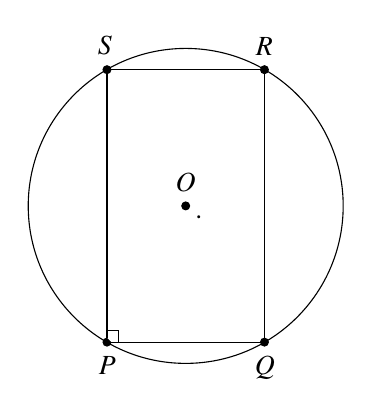
\begin{tikzpicture}
[scale =0.5,>=stealth,point/.style = {draw, circle, fill = black, inner sep = 1pt},]
\node (P) at (-2,-3.46)[point,label=below :$P$] {};
\node (Q) at (2,-3.46)[point,label=below :$Q$] {};
\node (R) at (2,3.46)[point,label=above :$R$] {};
\node (S) at (-2,3.46)[point,label=above :$S$] {};
\node (O) at (0,0)[point,label=above :$O$] {};
\draw (0,0) node [below right] {.} circle (4);
\draw (P)--(Q);
\draw (Q)--(R);
\draw (R)--(S);
\draw (S)--(P);

\tkzMarkRightAngle[fill=white!45,size=.3,mark=](S,P,Q)
\end{tikzpicture}
\end{document}
\end{center}
\item PQ = 2cm and PS = 4cm, radius = 4\\

\item \textbf{Calculation}
\begin{align*}
a = 2\\
c = 4\\
b = \sqrt{c^2} - a ^2\\
b = 3.46
\end{align*}
PQ =2\\
PS = 4\\

\includegraphics[scale=.4]{./figs/QUAD_P.eps}

\begin{lstlisting}
https://github.com/pratibha444/GEOMETRY/blob/master/figs/CYCPA.tex
\end{lstlisting}
\begin{lstlisting}
https://github.com/pratibha444/GEOMETRY/blob/master/CODES/quad/QUADP.py
\end{lstlisting}

\textbf{To prove} : PQRS is a rectangle\\

\textbf{Proof}: \\

\item $\angle$P = $\angle$R (opposite sides of parallelogram are equal)\\
\item $\angle$P + $\angle$R = 180$\degree$ (sum of opposite angles of a cyclic quadrilateral is 180$\degree$)\\

\item 2$\angle$P = 180$\degree$\\
\item$\angle$P = 90 $\degree$\\
Hence PQRS is a rectangle as in rectangle one angle is 90$\degree$.\\
\end{itemize}



\textbf{Triangle excercise}\\


\item Sides AB and AC of $\triangle$ABC are extended to points P and Q respectively.Also,$\angle$PBC $<$ $\angle$QCB.Show that AC$>$AB .
%Code by GVV Sharma
%December 6, 2019
%released under GNU GPL
%Drawing a right angled triangle

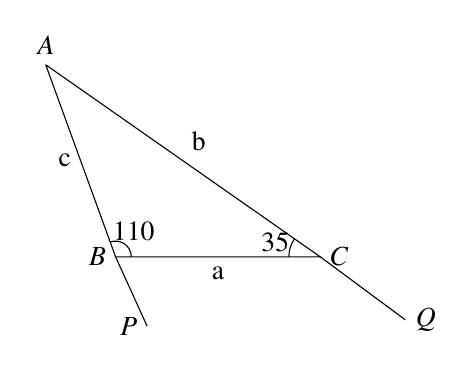
\begin{tikzpicture}[scale=0.4]

%Triangle sides
\def\a{6.5}
\def\c{6.5}
\def\b{10.64}

%Marking coordiantes
\coordinate [label=above:$A$] (A) at (-2.22,6.10);
\coordinate [label=left:$B$] (B) at (0,0);
\coordinate [label=right:$C$] (C) at (6.5,0);
\coordinate [label=left:$P$] (P) at (1,-2.2);
\coordinate [label=right:$Q$] (Q) at (9.2,-2);

%Drawing triangle ABC
\draw (A) -- node[left] {$\textrm{c}$} (B) -- node[below] {$\textrm{a}$} (C) -- node[above,,xshift=2mm] {$\textrm{b}$} (A);\draw (B)--(P);
\draw (C)--(Q);
%Drawing and marking angles
\tkzMarkAngle[arc=l,size=1,color=black](A,C,B)
\tkzLabelAngle[pos=1.5](A,C,B){\rotatebox{360}{$35$}}

\tkzMarkAngle[fill=white!40,size=0.5cm,mark=](C,B,A)
\tkzLabelAngle[pos=1](C,B,A){\rotatebox{-360}{$110$}}

\end{tikzpicture}


\begin{itemize}
\item a= 6.5,b=6.5,c=10.64\\
\item $c^2$ = $b^2$ + $a^2$ - 2abcos(B)\\
\item cos(C)= -($\frac{c^2 - b^2 -a^2}{2ab}$)\\
\item cos(C) = 35$\degree$\\
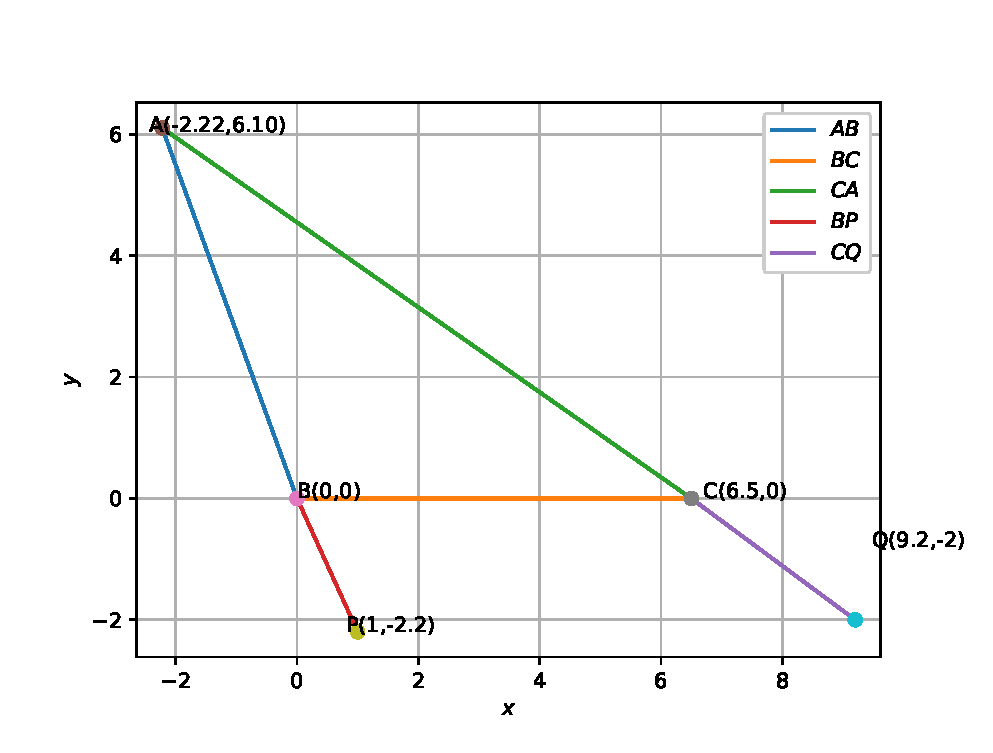
\includegraphics[scale=.4]{./figs/NEWTRI.eps}
\begin{lstlisting}
https://github.com/pratibha444/GEOMETRY/blob/master/figs/TRI_EX.tex
\end{lstlisting}
\begin{lstlisting}
https://github.com/pratibha444/GEOMETRY/blob/master/CODES/triangle/TRI_ISOP.py
\end{lstlisting}
\item \textbf{Given} : P and Q are extended to AB and AC respectively.\\
And $\angle$PBC $<$ $\angle$QCB --(1)\\
So,\\
$\angle$PBC + $\angle$ABC = 180$\degree$  \\
$\angle$QCB + $\angle$ACB = 180$\degree$  \\
$\angle$PBC = 180 - $\angle$ABC --(2)\\
$\angle$QCB = 180 - $\angle$ACB --(3)\\

By substituting the value of $\angle$PBC and $\angle$QCB in equation 1 \\

180 - $\angle$ABC $<$ 180 - $\angle$ACB\\
-$\angle$ABC $<$ -$\angle$ACB\\

multiplying both the sides by '-'\\

-(-$\angle$ABC) $>$  -(-$\angle$ACB)\\
$\angle$ABC $>$ $\angle$ACB
  
 (sides opposite to greater angle is longer)\\
\end{itemize}






\textbf{Miscellaneous Exercises}\\

\item The length of the
minute hand of a clock is 14 cm. Find the area
swept by the minute hand in 5 minutes.\\
\begin{itemize}
\item \textbf{Solution} :
\item Given r = 14 \\

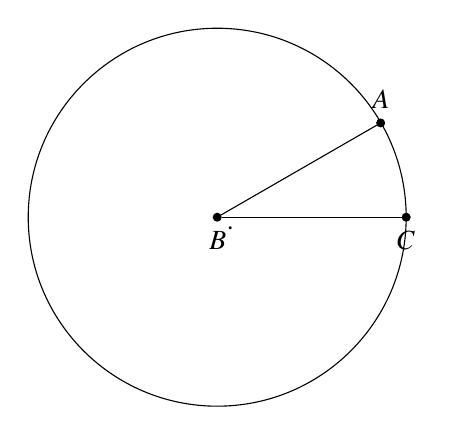
\begin{tikzpicture}
[scale =0.3,>=stealth,point/.style = {draw, circle, fill = black, inner sep = 1pt},]
\node (B) at (0,0)[point,label=below :$B$] {};
\node (C) at (8,0)[point,label=below :$C$] {};
\node (A) at (6.92,3.99)[point,label=above :$A$] {};
\draw (0,0) node [below right] {.} circle (8);
\draw (B)--(A);
\draw (B)--(C);
\end{tikzpicture}


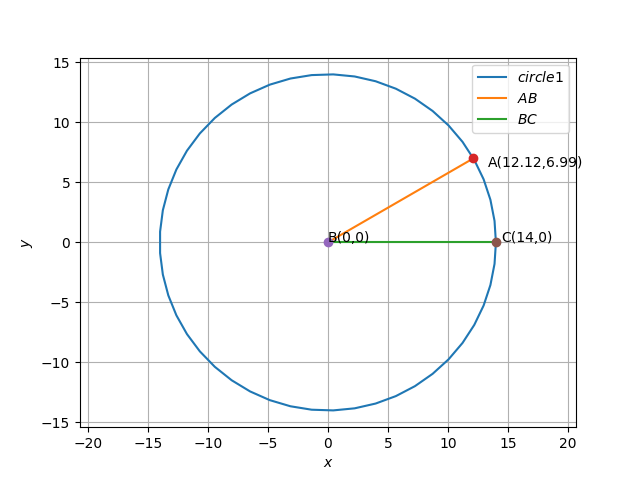
\includegraphics[scale=.6]{./CODES/quad/MISC.png}


 \item In 60 minutes minute hand covers  360$\degree$\\
For 5 minutes 6$\degree$ $\times$ 5 = 30$\degree$ 
\item Here $\theta$ = 30 $\degree$ and r = 14cm\\
\item Area of sector = $\frac{\theta}{360}$ $\times$ $\pi$ $r^2$
	=51.31$cm^2.$\\
	

	
\begin{lstlisting}
 https://github.com/pratibha444/GEOMETRY/blob/master/figs/clock.tex
 \end{lstlisting} 
 \begin{lstlisting}
https://github.com/pratibha444/GEOMETRY/blob/master/CODES/newclock.py
\end{lstlisting}
\end{itemize}             





\textbf{Quadrilateral construction}\\

\item Can you construct a quadrilateral PQRS with PQ=3, RS=3, PS=7.5, PR=8 and SQ=4?\\
\begin{itemize}
\item \textbf{Given}:  Quadrilateral PQRS with PQ = 3 cm RS =  3 cm PS = 7.5 cm and SQ = 4 cm\\

\item We know from triangle inequality theorem that sum of any two sides is greater than the third side ,\\
\item But here we have PQ = 3 cm PS =  7.5 cm SQ = 4 cm ( AS we get PQS triangle in quadrilateral PQRS where PQ and PS are sides and SQ is diagonal of quadrilateral . \\

And\\

PQ + SQ = 3 + 4 = 7\\

and\\

PS = 7.5 , So\\

PQ + SQ $<$PS ,\\
 But that equation is not true for another triangle.\\
So, we can't construct the given quadrilateral.
\end{itemize}





\end{enumerate}
\end{document}
